As a closing remark, let us briefly consider the question of \textit{what can and cannot be computed} with our logic language. On the surface our logic language looks very different from other programming languages such as, say, Java or F\#. Does this difference translate into higher or lower expressive power? In this chapter, we briefly and informally explore questions about the expressive power of different programming languages and programming paradigms. 

We will do so to justify the importance of programming languages and appropriate formalisms, but not for the purpose of expressing constructs that cannot be expressed into the other formalisms: rather, different languages and formalisms allow \textit{human users} to better reason, and as such do offer a different perspective on the same object (the set of all programs) which lets some different properties emerge better.

We will begin by discussing intrinsically hard problems that cannot have an algorithmic answer. These problems make up the boundaries of computability, and as such if we could\footnote{Spoiler alert: we can noooooooooooooooooooot!} define a formalism that solves one of this problems algorithmically then we would have found something that is intrinsically more expressive than the formalisms and languages that we use now.


\subsection{Halting problem}
We will now explore the simple question: \textit{are there limits to what can be computed?} In order to effectively manipulate programs we build a way to translate an arbitrary formula within some formalism into a natural number, that is we show a way to encode arbitrarily complex data structures into simpler objects that are easier to manipulate. 

This means that any statement within our formalism is now a natural number, and thus we have an isomorphism between ``properties of statements'' $\Leftrightarrow$ ``properties of numbers'', but ``properties of numbers'' are easier to determine algorithmically because we do not need to define data structures. 

\paragraph{Gödel numbering}
There are many ways to define such an encoding. We present Gödel's original encoding from many decades ago, mostly for historical reasons\footnote{A nice side-effect is that this encoding still works, which in a world of short-lived, superficial technological innovation where stuff stops working after a couple of years might seem strange. ``Should we not use something new and shiny?'', I hear you say: ``no.''}

We assign a unique natural number to each basic symbol in our language, for example:
\begin{itemize}
\item \texttt{if} $=0$
\item \texttt{var} $=1$
\item \texttt{,} $=2$
\item ...
\end{itemize}

Given any formula $x_1,x_2,\dots,x_n$, $x_i$ where each $x_i$ is a symbol with associated a number from the list above, we define the encoding function:

$$enc(x_1,\dots,x_n)=2^{x_1} \cdot3^{x_2} \cdot \dots \cdot p_n^{x_n}$$

where $p_n$ is the $n$-th prime number. This means that we encode the $i$-th symbol of the sequence as the exponent of the $i$-th prime number. According to the fundamental theorem of arithmetic, we can always extract back the original sequence with a finite number of steps.

For example, in a specific Gödel numbering, the Gödel number for $0$ could be $6$, and the Gödel number for $=$ could be $5$. Thus, in such a system, the Gödel number of formula $0 = 0$ would be $2^6 \times 3^5 \times 5^6 = 243000000$.


\paragraph{Halting}
Let us now consider the halting problem itself. Consider the problem of determining whether a program \texttt{i} terminates on input \texttt{x}. We can formulate this problem as finding function $h(i,x)$ that returns:

\begin{itemize}
\item $1$ if program $i$ terminates on input $x$
\item $0$ otherwise
\end{itemize}

Since we wish to automate this process, we want to find a way to translate function $h(i,x)$ into some program. For this to be possible, then function $h$ needs to be \textit{total} and \textit{computable}. A function is total if, for every input, it gives back a result. Trivially, function $h$ is defined so as to always return either $0$ or $1$, therefore it is total by definition. A function is computable if it can be encoded into a Turing machine or any equivalent formalism such as the $\lambda$-calculus. We shall further discuss these formalisms later, but for the moment let us treat them as mathematically flavoured assembly languages.


We will now show\footnote{\textit{Show} in this case is meant in the informal sense.} a shocking result: no arbitrary total computable function $f$ can be equal to $h$, and we will do so by constructing a counter example. The outline of the proof is as follows:
\begin{itemize}
\item we consider an \textit{arbitrary} total computable function $f$
\item we construct a partial but computable function $g$ that is based on $f$
\item we feed $g$ into $h$ (the halting function) and show that $f \neq h$
\item since $f$ was an \textit{arbitrary} total computable function, then there exists no total computable function $f = h$
\end{itemize}

Let us now consider an arbitrary total computable function $f$ in two arguments. We then define partial computable function $g(i)$ so that it returns:
\begin{itemize}
\item $0$ if $f(i,i)=0$
\item $\uparrow$ otherwise
\end{itemize}

Note that in the above, $\uparrow$ denotes no or undefined return value. This is allowed, as $g$ was meant to be a partial function. Not returning a value in practice amounts to infinite looping or (tail-)recursion, which effectively prevents a function from returning anything.

Since we chose $f$ to be totally computable, then as a consequence $g$ is will also be computable. We could formulate the above as follows in the logic programming language defined so far:

\begin{lstlisting}
f i i => 0
-----------
g i => 0
\end{lstlisting}

As long as \texttt{f i i} is also defined within the same program and always returns a result, then the above is a valid formulation within our language.

Since $g$ is computable, albeit partial, we can give a program computes $g$ and encode it with Gödel's numbering into $e_g$.

Let us now consider what happens if we give $e_g$ \textit{twice} to function $h$. $h(e_g,e_g)$ will return:

\begin{itemize}
\item $f(e_g,e_g)=0 \rightarrow g(e_g)=0 \ \rightarrow h(e_g,e_g)=1$
\item $f(e_g,e_g)=1 \rightarrow g(e_g)=\uparrow \ \rightarrow h(e_g,e_g)=0$
\end{itemize}

The above means that whatever $f$ returns, then $h$ returns something else. This means that $h \neq f$, but since $f$ was an \textit{arbitrary} total computable function, then $h$ is different from it and thus $h$ is different from all total computable functions.

The consequence of this is that $h$ is not computable, that is we cannot encode it within a Turing machine, $\lambda$-calculus, etc.

Not all hope is lost, because even if we cannot give a function $h$ that always answers \texttt{yes} or \texttt{no}, nothing stops us from  building an \textit{approximated} version of it. For example, we might restrict ourselves to solutions such as:
\begin{inparaenum}[\itshape i\upshape)]
\item a partial function, that may sometimes loop forever;
\item a function that can also return no answer, such as \texttt{unknown};
\item a function that gives probabilistic answers;
\item ...
\end{inparaenum}

We will focus on approximation techniques (even though not applied to the halting problem itself but one of its cousins) in later chapters.


\subsection{Some desperate grasping}
A reader with an active imagination might, at this point, be trying to find reasons why this does not really apply to his or her experience with programming. After all, this might just be an isolated incident, and most interesting things hopefully remain easily doable, right?\footnote{Yeah, you wish: this chapter goes from bad to worse, so giving up hope now will save you from depression further down the road. Sorry.}

Unfortunately for us, the mere fact that we cannot solve the halting problem really means that we cannot solve many hardcore problems that would make the life of programmers much easier.\footnote{This is actually the only silver lining: insightful programmers cannot be automated away, and will never be out of a job. Up yours, robotics!}

Some examples of problems that cannot be solved automatically as a consequence of the halting problem are:
\begin{itemize}
\item \textbf{EQUIVALENCE PROBLEM} Given two programs, test to see if they are equivalent.
\item \textbf{SIZE OPTIMIZATION PROBLEM} - Given a program, find the shortest equivalent program.
\item \textbf{GRAMMAR PROBLEM} Given two grammars, find out whether they define the same language.
\item ...
\end{itemize}

All of the problems above cannot be solved, because solving them would make it possible to also solve the halting problem.\footnote{This proof strategy is known as \textit{reduction}, because it reduces one problem to another one, showing that solving the first implies solving the second or vice-versa.}

For example, consider the equivalence problem. Suppose (\textit{ad absurdum}\footnote{A proof based on \textit{reductio ad absurdum} assumes something that we suspect to be false and shows that from this assumption stems a clear contradiction against some previously established fact.}) we have a function \texttt{equivalent} that is capable of reliably testing whether two programs are equivalent on some input. We will now show how we could use this equivalence test to determine whether or not a program \texttt{P} halts on input \texttt{i}. To do so, we construct a new program \texttt{Q} that works precisely like \texttt{P}, but which returns \texttt{1} whenever \texttt{P} would return something. This would be equivalent to simply ignoring the result of \texttt{P}, for example:

\begin{lstlisting}
P => res
---------
Q => 1
\end{lstlisting}

We now construct a new, trivial program \texttt{T} that always returns \texttt{1}:

\begin{lstlisting}
-------
T => 1
\end{lstlisting}

We now use our function \texttt{equivalent} on \texttt{Q} and \texttt{T}. If \texttt{Q} and \texttt{T} are equivalent, then this means that \texttt{Q} halts, therefore \texttt{P} halts as well. Since we know that we cannot solve the halting problem, then our original hypothesis that we have a total, computable \texttt{equivalent} function was absurd. 

Similar proofs can be set up for all problems that involve the automated, reliable determination of complex properties of programs. This generalization is known as \textit{Rice's Theorem}, which states that, for any non-trivial property of partial functions, there is no total computable function that decides whether an algorithm computes with that property. Here, non-trivial means that it is a property that holds for some but not all partial computable funcctions.

\textit{Rice's Theorem} is quite a dramatic result, because it ultimately guarantees that no fully reliable algorithm will ever be able to perfectly optimize a program for speed or size, no compiler will be able to verify the correctness of programs, etc.\footnote{This is the permanent guarantee of employment for at least some programmers that was mentioned in a previous footnote. Yay!}


\paragraph{Computers are really finite}
The last, desperate attempt at solving the halting problem could be done by a self-appointed smart person that observes how computers are not really correct implementations of Turing machines. In particular, it could be noticed how memory in a modern computer is actually finite, and thus a modern computer is really a large state machine. A non-terminating program will eventually run out of new memory states to explore, and revert back to an older memory state. Thus by tracking all memory states seen so far by the program we can determine if the program does not halt after \textit{enough steps} to explore all the possible memory states. But \textit{how large of a state machine are we talking about}, and thus how many is \textit{enough steps}? Consider a computer with just one gigabyte, which for practical purpose we will assume to be $10^9$ bits. This means that we would need to perform at most $2^{10^9}$ steps, in order to check all possible bit configurations. Now $2^{10^9}$ is indeed a finite number, if one is into this kind of distinction, but as far as finite numbers go it is sufficiently big to make any concrete implementation impossibly slow. It is safe to assume that the civilization of the creator of the program will likely be dead well before the program finishes running. Whether we choose to use a computer with less memory will still be pointless, since even for a computer with one kilobyte we would need to perform at most $2^{10^5}$ steps, which is still a prohibitively large number. Whoever tries to run such a program will not likely see the result within his or her lifetime.

Of course modern computers have far more memory, and programs are often connected to the Internet. This means that the actual program running is a large distributed program which state is far larger and distributed, further making any ``finite memory'' argument completely unusable in practice.

\subsection{Some equivalences and translations}
Someone might wonder if it is possible to define some formalism that solves the halting problem by simply shifting the perspective. Perhaps there exists some new way to formulate new programming languages that do not suffer from this issue?

The basic formalisms of computing are two well-known theoretical programming languages, which are \textit{Turing machines} on one hand and the $\lambda$\textit{-calculus} on the other. Already during the previous century\footnote{For the perspective of future readers, we are talking about the 1900's.} it was discovered that these languages are \textbf{isomorph}, that is they can both express exactly the same programs, and neither can do something that the other cannot. This shocking result was brought about by the presence of translation routines that allow to translate \textit{any} Turing-machine program in a semantically equivalent\footnote{That is which performs exactly the same computation.} $\lambda$-calculus program, and vice-versa.

Without diving into the details of these formalisms, it is possible to observe that we have not yet found a way to escape the circle. For example, we could notice that in our case, there exists a chain of translations that goes as follows:

\begin{lstlisting}[mathescape=true]
$\lambda$-calculus => F# => our logic language
\end{lstlisting}

Now if we can show that we can implement the $\lambda$-calculus into our logic language, then we have ``closed the circle''. The grammar of the language is made up of three simple terms: 
\begin{inparaenum}[\itshape i\upshape)]
\item identifiers (intuitively similar to variables), which are simply strings wrapped by \texttt{\$};
\item lambda terms (intuitively similar to function declarations), which take the form \texttt{\textbackslash \$x -> TERM};
\item applications (intuitively similar to function calls), which take the form \texttt{TERM | TERM}.
\end{inparaenum}

This syntax is defined in our language as:

\begin{lstlisting}
Data [] [] "$" [<<string>>] Priority 10 Type Id
Data [] [] "\" [Id Arrow Term] Priority 9 Type Term
Data [] [Term] "|" [Term] Priority 8 Type Term
\end{lstlisting}

Of course an identifier is also a term, thus:

\begin{lstlisting}
Id is Term
\end{lstlisting}

The arrow is not strictly needed, but it is aesthetically pleasing in that it helps distinguish a function arguments from its body:

\begin{lstlisting}
Data [] [] "->" [] Priority 0 Type Arrow
\end{lstlisting}

Execution\footnote{This is just one of the many possible evaluation strategies for the $\lambda$-calculus, which is perhaps the most intuitive for a programmer with a traditional imperative background.} of a program within the calculus is quite simple: whenever we apply a lambda term (the function being called) to another term (the argument), then the result \textit{is the body of the function called where the function parameter has been replaced by the value of the argument}.

Execution of any term which is not the application of a lambda term to something else simply does nothing:

\begin{lstlisting}
---------
$x => $x

---------------
\$x -> t => \$x -> t

-----------------
$x | u => $x | u
\end{lstlisting}

Nested applications are solved from the right to the left:

\begin{lstlisting}
w => w'
u | v => uv
uv | w' => res
-------------------
(u | v) | w => res
\end{lstlisting}

Finally, applications of lambda terms to other, arbitrary terms instance \textit{substitutions}. Substitutions are of the form \texttt{TERM with \$x as TERM}, indicating that we are replacing variable \texttt{\$x} with some other term:

\begin{lstlisting}
Data [] [Term] "as" [Term] Priority 6 Type Where
Data [] [Term] "with" [Where] Priority 5 Type With
\end{lstlisting}

To evaluate such an application, which is of the form \texttt{\textbackslash\$x -> t | u}, we first evaluate \texttt{u} into \texttt{u'}, and then replace \texttt{\$x} with \texttt{u'} within \texttt{t}:

\begin{lstlisting}
u => u'
t with ($x as u') => t'
-----------------------------------
\$x -> t | u => t'
\end{lstlisting}

If we find the variable we needed to replace with term \texttt{u}, then instead of the variable we return \texttt{u} itself:

\begin{lstlisting}
  x == y
  ---------------------
  $y with $x as u => u
\end{lstlisting}

If we find a different variable than the one we needed to replace, then we return the variable unchanged because no replacement is possible:

\begin{lstlisting}
  x != y
  ----------------------
  $y with $x as u => $y
\end{lstlisting}

If we find a redefinition of the variable we were replacing, then we stop the replacement procedure as the variable we were replacement has been shadowed and a new one becomes active in the new scope created:

\begin{lstlisting}
  x == y
  ----------------------------------
  \$x -> t with $y as u => \$x -> t
\end{lstlisting}

If we find a variable definition for a new variable which is not the one we were replacing, then we proceed with replacement within the body of the function definition:

\begin{lstlisting}
  x != y
  t with $y as u => t'
  -----------------------------
  \$x -> t with $y as u => \$x -> t'
\end{lstlisting}

If we find an application, then we perform the replacement within both terms of the application and return the resulting application:

\begin{lstlisting}
  t with $x as v => t'
  u with $x as v => u'
  --------------------------------
  (t | u) with $x as v => t' | u'
\end{lstlisting}

Consider now the evaluation of a simple term such as:

\begin{lstlisting}
-----------------------------
(\$"x" -> $"x") | $"y" => ?
\end{lstlisting}

The first step of evaluation tries to evaluate term \texttt{\$"y"}, and then replace \texttt{\$"x"} with the result of this evaluation:

\begin{lstlisting}
$"y" => u'
$"x" with $"x" as u' => t'
--------------------------------------
(\$"x" -> $"x") | $"y" => t'
\end{lstlisting}

The evaluation of \texttt{\$"y"} simply returns \texttt{\$"y"} itself, because a variable always evaluates to itself:

\begin{lstlisting}
$"y" => $"y"
$"x" with $"x" as $"y" => t'
-----------------------------
(\$"x" -> $"x") | $"y" => t'
\end{lstlisting}

Evaluation then proceeds to the next premise, which is a replacement of the right variable

\begin{lstlisting}
$"x" == $"x"
t' := $"y"
----------------------------------------
$"x" with $"x" as $"y" => t'
--------------------------------------
(\$"x" -> $"x") | $"y" => t'
\end{lstlisting}

We can now begin the unwinding procedure, which after just one step returns:

\begin{lstlisting}
(\$"x" -> $"x") | $"y" => $"y"
\end{lstlisting}

Which is precisely the answer we expected.


By implementing the $\lambda$-calculus then we have shown how on one hand our language \textit{is not more powerful} than any of the well-known formalisms of programming, but on the other hand we have shown how our language \textit{is not less powerful} than any of the well-known formalisms of programming.

This being exactly as powerful as the $\lambda$-calculus or Turing machines is known as the \textbf{Church-Turing equivalence}, and is the best known way to define the expressive power of programming. The existance and apparent inescapability of the Church-Turing equivalence suggests that there is no preferred encoding which ``unlocks'' impossible problems such as the halting problem, therefore making them computable.



\section{Conclusion}
%One might be tempted to look outside of programming
%Maybe mathematical encodings offer a solution?

%Apparently we have the same issue
%Exemplified by Russel's paradox
%$R = \{ x . x \notin x \}$
%\begin{itemize}
%\item $R \in R$?
%\item $R \notin R$?
%\end{itemize}

%A devastating generalization of Russel's paradox
%First incompleteness theorem:
%\begin{itemize}
%\item no consistent system of axioms whose theorems can be listed by an ``effective procedure''
%\item capable of proving all truths about the relations of the natural numbers
%\item For any such system, there will always be statements about the natural numbers that are true, but unprovable
%\end{itemize}
%Proven by constructing self-referencing objects

%the direct relationship between computer programs and mathematical proofs
%observation that two families of formalisms that had seemed unrelated are in fact structurally the same kind of objects
%\textit{a proof is a program, the formula it proves is a type for the program}
%\textit{running a program is equivalent to ``simplifying'' a theorem}

%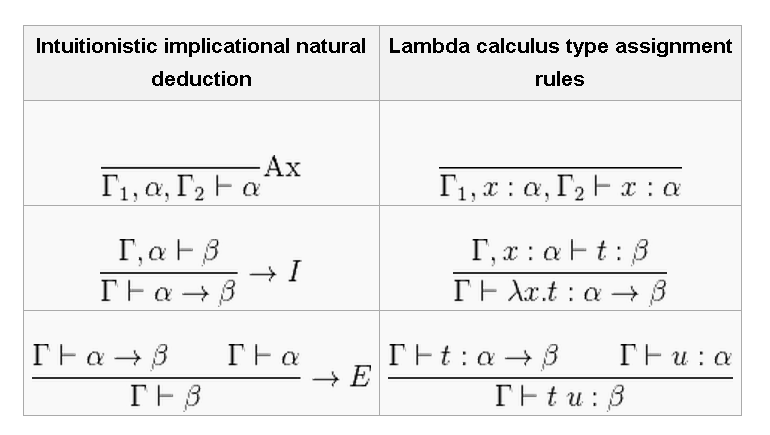
\includegraphics[width=11cm]{pics/curryhoward.png}



What we have seen so far leaves us with a new perspective on computation. No matter what language we choose, there seems to be a hard limit on what is possible to compute. This means that:

\begin{inparaenum}[\itshape i\upshape)]
\item programming languages all represent, at their core, the same set of objects (the set of all programs);
\item some problems cannot be solved with an automated solution, independently of the programming language;
\end{inparaenum}

Why is the search for new programming languages interesting thus, if they allow us no more expressive power? In reality, programming languages have more or less expressive power, but not because of what they can compute, but because they allow a clearer interaction with the \textit{humans} that use them. As A. Whitehead\footnote{A famous mathematician for as far as fame goes for mathematicians.} said in ``The Importance of Good Notation'', in his book \textit{An Introduction to Mathematics}:

\begin{displayquote}
[...] by the aid of symbolism, we can make transitions in reasoning almost mechanically by the eye, which otherwise would call into play the higher faculties of the brain.

[...]

One very important property for symbolism to possess is that it should be concise, so as to be visible at one glance of the eye and to be rapidly written. 

[...]

It is interesting to note how important for the development of science a modest-looking symbol may be. It may stand for the emphatic presentation of an idea, often a very subtle idea, and by its existence make it easy to exhibit the relation of this idea to all the complex trains of ideas in which it occurs. For example, take the most modest of all symbols, namely, 0, which stands for the number zero. The Roman notation for numbers had no symbol for zero, and probably most mathematicians of the ancient world would have been horribly puzzled by the idea of the number zero. For, after all, it is a very subtle idea, not at all obvious. A great deal of discussion on the meaning of the zero of quantity will be found in philosophic works. Zero is not, in real truth, more difficult or subtle in idea than the other cardinal numbers.
\end{displayquote}

Thus programming languages make it easier to express some aspects of thoughts rather than some others, and by emphasizing concepts such as correctness or reliability we can dramatically change the impact of the language on the thought process of the programmer.


About the unsolvable problem, also here is some silver present. Even though we cannot provide a perfect solution to these problems, nothing forbids us from building partial solutions that allow for uncertainty. We can thus always build a program that can answer questions about termination, correctness, or equivalence between programs with answers taken from the set \texttt{yes}, \texttt{no}, and \texttt{unknown}. The ability to return \texttt{unknown} suddenly makes the program possible to build, therefore exchanging some precision with implementability. 

The challenge that arises from this is thus that of reducing the number of programs for which our analyser returns \texttt{unknown} so that it is as small as possible. Not only do we wish to reduce the number of uncertain programs, we might also find it acceptable to have our analysis ``give up'' for programs where the flow of control is complex or hard to follow, in the assumptions that these programs, even when working, are not acceptable for being too confusing\footnote{If a program is confusing for a carefully built analyser, imagine what it does to the brain of Bob, a 20-something junior programmer who just came out of a coding bootcamp and sits two cubicles over.}. Theoretical frameworks such as dependent types, model checking, and abstract interpretation (just to name a few) are written with the goal in mind of standardizing the concepts of approximated analysis of computer programs, precisely with the goal of providing an incomplete, but still useful, solution to problems such as halting.
